\section[How can control engineers help agriculture?]{Sidebar: Key control problems in agriculture}\label{sb:ag}


Shortage of qualified human labor is a key challenge facing farmers \cite{richards2018immigration,hertz2013there}, leading to smaller profit margins, and preventing the adoption of truly sustainable agricultural practices. Lack of timely available labor was a principle reason behind the tens of millions of dollars of unharvested fruits and vegetables that rotted in California farms in 2017 \cite{guthman2017paradoxes,RN4026}.  Labor shortages can be a major barrier to more sustainable agricultural practices that are more labor intensive.

For example, more sustainable alternatives to prevalent methods of agriculture that would not need large amounts of chemicals and other inputs, such as perennial polycultures (mixed species of fruit- and nut-producing trees and shrubs \cite{lovell2017temperate}, see Figure \ref{fig:polycultures}), are currently impractical at scale with current agricultural equipment. Polyculture systems can leverage co-habitation of mutually beneficial plants (and animals, insects, or microbiomes) to create a more sustainable engineered ecosystem. Labor shortage has become a primary barrier to adoption of this sustainable agricultural alternative \cite{RN4017,RN4018}.  


One way to address the challenges of labor shortages in agriculture is by creating new robotic technology that can work in harsh, uncertain, and dynamically changing field environments. 
Here we outline some of the fundamental challenges in autonomy, estimation, and control that the controls community can help overcome to enable the future of agricultural robotics, and relate it with the problem of spatiotemporal function estimation studied in this paper:

\textbf{Persistent multi-agent autonomy under partial observability}:  The digital farm of the future will employ teams of distributed heterogeneous agents to autonomously manage, optimize, and harvest large acres of diverse crops across the entire season without encumbering humans. This level of autonomy in unstructured field environments is out of reach of the current state-of-the-art which requires constant human monitoring and oversight, especially in the presence of change or unforeseen events. Efficient and reliable control will be central to the success of these robots. Small below-canopy robots (e.g. Figure \ref{fig:terrasentia} \cite{kayacan2018embedded}) will need to provide precision care including pruning, weeding, and re-seeding without damaging plants or causing soil compaction. Deployed at scale, these robots can not only make large scale organic farming practical, but also enable enhanced breeding through  field-scale phenotyping \cite{kayacan2018embedded,mueller2017robotanist,virlet2017field}. \textit{The big controls challenge here is in making decisions over large spatiotemporal scales with information obtained from a few stationary and mobile sensors which can only partially observe the environment at any given time}. The work pursued in this paper lays a foundation towards this problem by enabling a team of agents to estimate the varying state of the environment. 

\begin{figure}
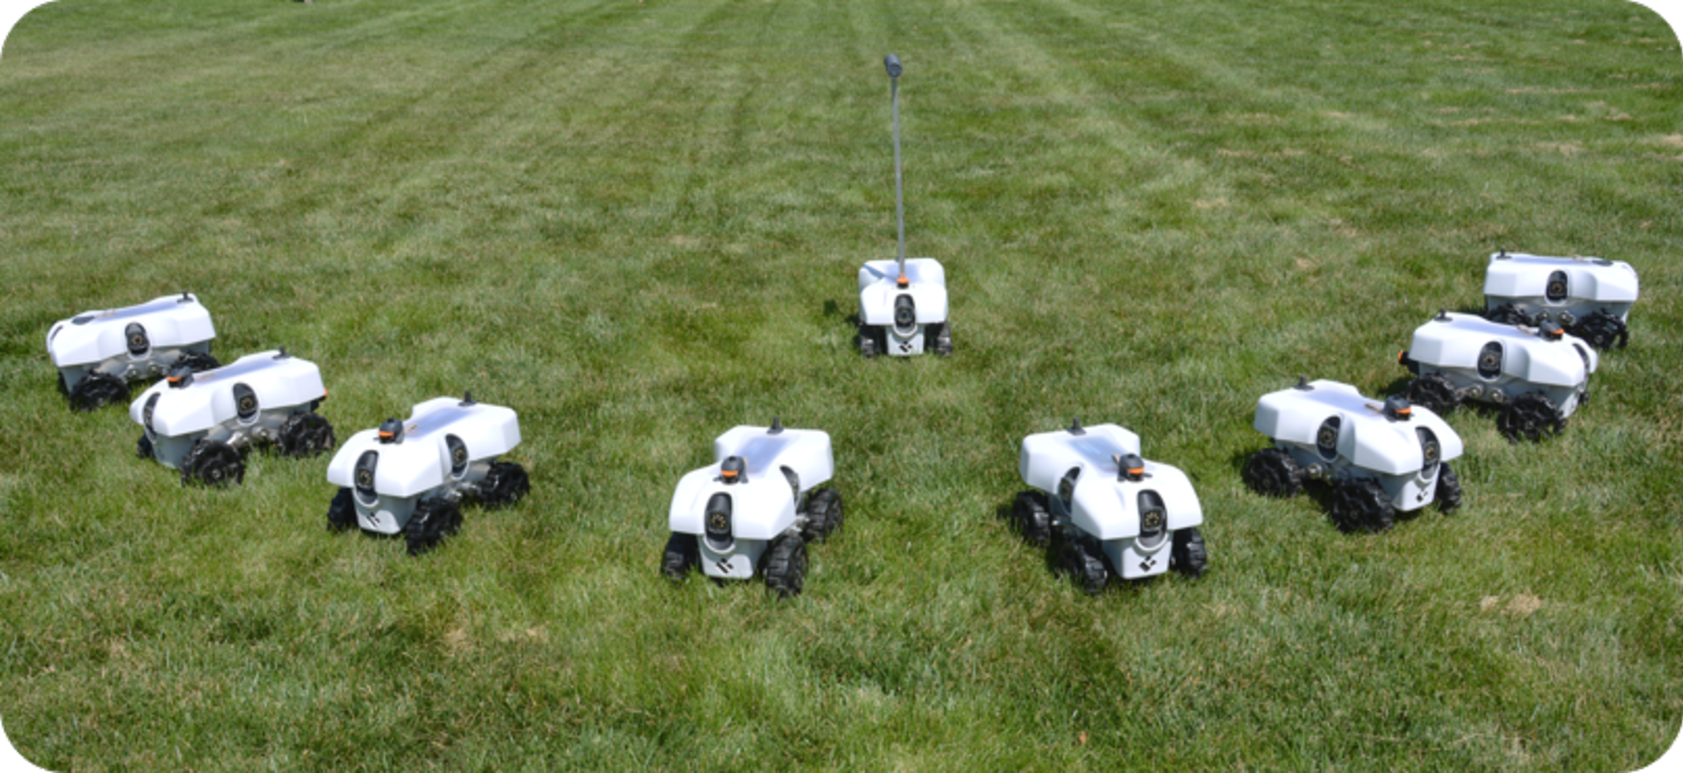
\includegraphics[width=\textwidth]{swarmbots}
\caption{The TerraSentia robots developed by Chowdhary's group at UIUC and commercialized by EarthSense inc. Agricultural robots such as these present exciting possibilities for distributed agricultural management with teams of compact, ultra-light, under-canopy robots equipped with advanced autonomy and machine learning. Such robots can fill the niche between large farm equipment and manual labor, as well as enable perennial polycultures, and closer to home,  they could also weed your garden! Advances in persistent multi-agent autonomy in harsh, changing, and uncertain environments driven by the controls community are driving such exciting possibilities of the future of agriculture.}
\label{fig:terrasentia}
\end{figure}


%\textbf{Soft robots}

\textbf{Dexterous and ubiquitous robotics for precise care} : The digital farm of the future will strive to eliminate costly inputs (chemicals, labor, energy, and knowledge) with low-cost, dexterous, and highly autonomous agricultural equipment \cite{pedersen2006agricultural}. Advances in \textit{soft} arms and grippers can enable robots that can have far better reach and dexterity around plants than robots equipped with traditional \textit{hard} industrial robotic arms. Soft arms, which are often actuated with pressurized tubes, can be far less expensive to manufacture and significantly lighter than their hard counterparts. On the other hand, soft arms can be slow to actuate and have limited payloads. To make soft robots practical, optimal feedback control techniques are necessary that work with conformal objects with very large degrees of freedom. In particular, soft arms tend to significantly deform under weight and behave quite differently when loaded with different payloads. Unlike hard arms, encoders are not sufficient to estimate the pose of the arm or the manipulator. Strain and angle sensors need to be positioned judicially to keep costs down, and image based feedback control will be necessary. The evolving Gaussian Process technique and the kernel observer techniques described in this paper could be utilized to create distributed observers for such soft systems.  

The complex interaction between closely-spaced diverse plant species in a polyculture results in both spatial and temporal dynamics as the plants grow and interact with each other. %in polyculture parameters, such as growth rate, plant phenology, and yield. 
Plant growth often exhibits hybrid dynamical systems behavior with rapid thresholded growth bursts followed by slow progression. The triggers for growth bursts are dependent on  environmental factors such as temperature, soil moisture, and sunlight reaching individual and cumulative thresholds, and complex interrelations between neighboring plants, soil chemistry, insects, and soil microbes. 

Simulating individual plant growth is an active area of research with many open questions in modeling and plant biology \cite{zhu2016plants}. Arguably, very high resolution plant growth models may not even be necessary for effective control of polycultures. Yet on the other hand, the  %TThere are many open problems in modeling 
 %Furthermore, plant growth follows sigmoidal phase transitions: even though  However, 
 existing models of plants and interactions with ecosystems \cite{Stehfest2007a,Foley1996a, Kucharik2003a,Friedl2010a, Rodrigues2010a, Nunes2013a} are not well suited for designing and managing polycultures because of the simplifying assumptions that are often made. A good balance could be struck with data driven machine learning models that have sufficient resolution for aggregate prediction over multiple spatiotemporal scales and are lightweight enough for control and decision making. With these models, predictive control strategies can be created that task teams of robots for management tasks. Furthermore, these predictive models can enable quantified mechanisms of design and planning of efficient agroecosystems.  
 Obtaining the required data to train these models and using them to create effective control techniques for managing profitable polycultures remains an exciting direction of future work where the controls community can help.
 
 The discussion in this sidebar was informed by many conversations with  crop scientists at UIUC. In particular, 
\textit{the authors wish to thank Prof. Stephen Long and Prof. Carl Bernacchi for insights on the phenotyping bottleneck and simulation of plants (\textit{crops-in-silico}), Prof. Adam Davis on inputs on the herbicide resistant weed crisis, and Prof. Sarah Lovell on sustainable agricultural production systems and perennial polycultures, as well as the members of the UIUC Center for Digital Agriculture} 

\begin{figure}[tbh]
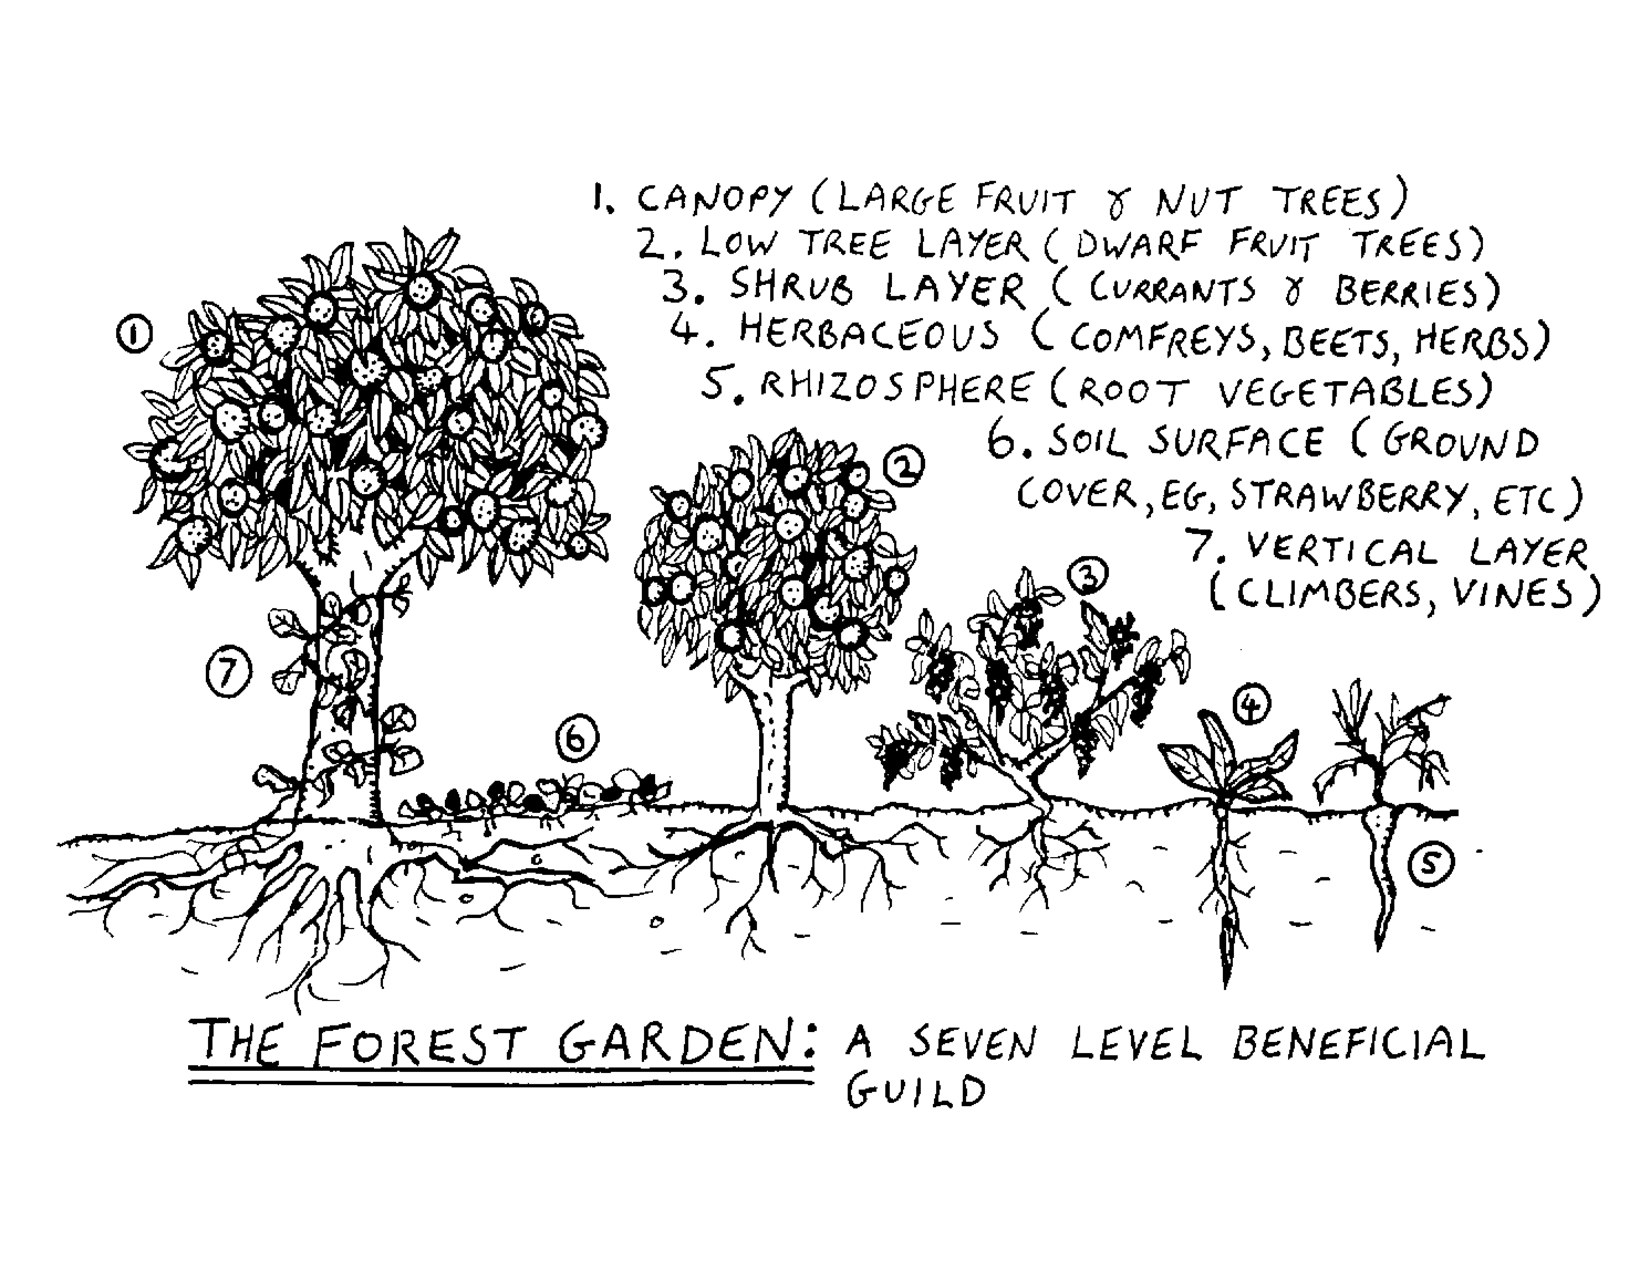
\includegraphics[width=\textwidth]{./figures/polyculture}
\caption{The seven layers of the forest garden. Polyculture agricultural production systems are designed ecosystems that can be more productive and sustainable than traditional monoculture systems. Managing such complex systems requires fundamental advances in robotics, spatiotemporal modeling, and control of complex biological processes, all areas where the control community can help. Figure source \cite{polyculture_fig}  see also \cite{rhodes2012feeding}.}
\label{fig:polycultures}
\end{figure}
